\documentclass[a4paper]{article}
\usepackage{amsmath}
\usepackage{amssymb}
\usepackage{fancyhdr}
\usepackage{a4wide}
\usepackage{geometry}
\usepackage[utf8]{inputenc}
\usepackage{graphicx}
\geometry{a4paper,left=2cm,right=2cm, top=3cm, bottom=3cm}
\usepackage{listings}

\newcommand{\titel}[1]{\fancyhead[C]{#1}}
\newcommand{\name}{\fancyhead[L]{Alexander Landmesser}}
\newcommand{\matrikel}{\fancyhead[R]{}}
\newcommand{\pl}{\hspace*{1cm}}
\begin{document}
\title{Verteilte Systeme}
\maketitle
\section{ØMQ}
\subsection{Verwendung}
\begin{itemize}
\item[1. Context:] Es muss für ØMQ ein Kontext erstellt werden (das Umfeld)
\item[2. Socket:] Es muss ein Socket in diesem Kontext erstellt werden
\item[3. Sockettyp:] Was für eine Art Socket wird benötigt (SUB/PUB etc.)
\item[4. Binding:] Socket an eine Adresse und einen Port binden (Remote, oder Lokale für listening)
\item[5.1 Receive] Receive (blockierend), besonderer Messagetyp
\item[5.2 Send] Send, gegebener Messagetyp ist zu füllen

\end{itemize}
ØMQ Buffert alle Nachrichten bis zu einem gewissen Grad. So werden auch langsamere Reader oder später registrierte Subscriber bedient, jedoch ohne versicherung, dass sie alle Nachrichten empfangen.
\subsection{Patterns}
\begin{itemize}
\item[Request-Reply] Synchrone Request-Reply Kommunikation
\item[Push-Pull] Sender erwartet keine Rückantwort (Push), Empfänger benutzen Pull, um Nachricht zu empfangen.\\
Kann benutzt werden, um Lasten zu verteilen, weil eine Nachricht nur höchstens eimal empfangen werden kann.
\item[Pub/Sub] Ein Publisher sendet Nachrichten mit bestimmten Tags, alle Subscriber empfangen alle Nachrichten, die den vorgegebenen Tags des Subscribers entsprechen.
\end{itemize}
\subsection{Transportvarianten}
\begin{itemize}
\item[ipc:] Interprozess, FIFO etc.
\item[inproc:] Socketkommunikation innerhalb eines Prozesses.
\item[mMulticast:] ØMQ unterstützt Multicast, wenn das Netzwerk es unterstützt.
\end{itemize}
\subsection{PlayØMQ, Broker}
Sources generieren Zufallszahlen und geben sie an den Broker.\\
Worker nehmen Zahlen aus dem Broker und prüfen auf Primzahl.\\
Sinks hören auf Nummern/Primzahlen.
Broker: Sendet einkommende Zahlen per Push-Socket an Worker, sendet Zahlen und Primzahlen per PUB-Socket
Source: Request Reply auf Broker.\\
Worker: Push/Pull $\rightarrow$ Parallelisierung der Berechnung \\
Sink: Subscriber, die auf den Broker "Subscriben", mit dem entsprechenden Tag (number/primzahl)
\subsubsection{Nachrichten}
Senden und Empfangen von Daten muss besonders behandelt werden, da Nachrichten erstellt werden müssen.\\
Nachrichten bestehen aus Tag (identifier Char) und Wert (long)
\subsubsection{Source}
Benötigt URL von Broker\\
Erstelle REQ (Request) Socket, der mit dem Broker verbindet.\\
Source generiert Zahlen, sendet sie an Broker und wartet, bis dieser den Empfang bestätigt hat.
\subsubsection{Broker}
Broker hat Sockets für REP (Reply) für Source, PUB (Publisher) für Sinks, PUSH für Worker.\\
Im Beispiel ist Endpoint eine Methode, die die Befehle zum Erstellen eines einfachen Sockets zusammenfasst.\\
Broker empfängt Zahl von Source, bestätigt dem Empfang, publiziert die Nummer, sendet sie an die Worker, wartet auf die Antwort und publiziert u.U. die Primzahl.
\subsubsection{Worker}
Verbindet per PULL und REQ (Request) Socket auf den Broker. \\
Empfängt vom Broker per PULL Zahlen, prüft diese und sendet sie u.U. per REQ an Broker. Wenn die Primzahl gesendet wird, muss der Worker wieder auf die Antwort (REPly) des Broker warten.
\subsubsection{Sink}
Erstellt SUB (Subscriber) Socket, über den er vom Broker Daten empfängt. \\
Beim Erstellen wird festgelegt, auf welche Tags der Subscriber hört.\\
\section{Verteilung von Last}

Kreative Lastverteilung: Verteilte Programmierung.\\
Mechanische Lastverteilung: Verteilung auf Rechner, gleiche Auslastung der verwendeten Rechner\\

Durch verteilte Rechner ist die "aktuelle Last" verzögert, um die Latenz zwischen A und B. A schickt also Last an B, auch wenn B inzwischen eine hohe Last erreicht hat.\\
Lösung: A kann anhand der verteilten Last merken, wie viel Last ungefähr an B vergeben wurde (wenn B Last nicht weitergibt).\\

Paketweitergabe:\\
\begin{itemize}
\item Wenn der Code lokal vorhanden ist, muss er kopiert werden (achte auf identische Pfadnamen etc.)\\
	Bei Netzwerklaufwerken geht Zeit verloren, da das Netzwerklaufwerk limitierende Bandbreite hat.
\item Verteiler schickt Programmcode mit (Große Datenmenge, Achtung Viren)

\end{itemize}

\subsection{Architektur}
Erstellen einer Lastmetrik: Welche Last hat ein Rechner, welche Last erzeugt ein Paket?\\
Verteilung der Last der beteiligten Rechner: Entscheidungsgundlage für Verteiler.\\
Verteilung des Lastpaketes auf gewählte Rechner: Welche Informationen müssen übertragen werden.\\
\subsection*{Lastmetriken}
\begin{itemize}
\item Prozessorauslastung (Anzahl Prozesse, CPU-Zeit)
\item Speicherauslastung (Bedarf etc.)
\item Kommunikationslast (IO, Netzwerk)
\end{itemize}
\subsubsection*{Pull}
Zieht Lastwerten an. (Unterforderte Rechner suchen Last)\\
Lastwert wird bei der Erzeugung eines Paketes ermittelt.\\
Varianten:
\begin{itemize}
\item[Von allen Rechnern:] Verteiler sendet Broadcast und fragt nach Last, alle Rechner antworten mit eignener Last.\\
	Verbesserung: Antowrt wird verzögert, je nach eigener Last. Damit antwortet der am wenigsten ausgelastete als erstes.
\item[Feste Teilmenge:] Erreriche bestimmte Worker
\item[Zufällige Teilmenge:]Frage zufällige Worker an
\end{itemize}
\subsubsection*{Push}
Lastwerte verteilen.  (Überforderte Rechner verteilen Last)\\

\subsection{Verteilungsverfahren}
Last sollte so verteilt werden, dass Rechen- und Speicherlast gleich verteilt ist und die Kommunikation möglichst lokal stattfindet.
\begin{itemize}
\item[Statisches Verfahren] Optimale Verteilung vor dem Start der Anwendung ermitteln.\\ 
Alle Bestandteile der Lastmetrik sind für alle Prozesse bekannt.\\
Findet häufig Anwendung, Last ist vorher meistens bekannt (Meterologie etc.)
\item[Dynamisches Verfahren] Ausführungsort wird für jeden Prozess ermittelt. 
	\begin{itemize}
	\item[Mit Migration] Migration heißt, die Adressräume und die Prozessstati zu übertragen. Es muss gewartet werden, bis alle Threads keine OS-Ressourcen mehr benutzen.\\
	Problem: Adressräume sind u.U. sehr groß. \\
	Lösung: Copy-on-Reference: Kopiere Adressen, wenn sie benötigt werden. (Reduziert Speicherlast auf Quellknoten nicht).
	\item[Ohne Migration] Hoher Aufwand die Lastverteilung zu bestimmen.
	\end{itemize}
\end{itemize}
Durchgesetzt hat sich \underline{Initial Placement}\\
Bei Paketentstehung Zielknoten bestimmen, im Extremfall zufällige Wahl.\\
Ist durchaus das schnellste Verfahren.\\
\subsection{Zeit bei Verteilung}
2 Möglichkeiten:
\begin{itemize}
\item 1. Synchronisieren der Uhren der Systeme
\item 2. Erstellung eines neuen Zeitmaßes
\end{itemize}
\subsubsection{Synchronisation der Uhren}
Es wird angenommen, dass jede Uhr ungenau ist und eine lineare Abweichung besitzen.\\
Ziel: Zeit innerhlab eines Rahmen halten und Abweichungen durch Synchronisation verhindern.\\
Ein System hat eine genaue Zeit, die an andere Systeme verteilt wird:\\
Die nachgestellten Uhren hinken immer ein wenig hinterher. \\
DCF77 erste Zeitsender in Offenbach, senden Zeitsignal über Langwelle. Pulst jede Sekunde, Zusatzdaten auf das Sekundensignal moduliert.\\
\textbf{Vergleich nach F. Christian}:\\
Client muss herausfinden, was die Laufzeit des Singals ist. Er speichert seine Zeit, wenn das Signal losgeschickt wird und wenn die Antwort empfangen wird. Der Client berechnet die Mitte aus Empfangszeit-Sendezeit, dieser Zeitpunkt wird auf die Zeit des Signals (Servers) gesetzt.\\
Lokale Uhr kann schneller/langsamer sein. Zurückstellen der Zeit ist unangenehm, deswegen werden Anti-Schaltmillisekunden eingeführt, die die Uhr bei Bedarf leicht abbremsen. Auch beim Vorstellen der Uhr werden meist Schaltmillisekunden verwendet.\\
\textbf{NTP}:\\
Server werden in Genauigkeitsstufen unterteilt, Stratum1 ist genau. Stratum 3 oder mehr ist inzwischen selten.\\
Lokale NTP Server ermöglichen eine sehr genaue lokale Zeit im Netzwerk. Die Uhr ist nicht unbedingt genau die Globalzeit, alle lokalen Systeme laufen aber synchron.\\
\subsubsection{Lamportzeit}
Bei jedem lokalen Ereignis "tickt" die logische Uhr. Lokale Ereignisse können Instruktionen oder spezielle Ereignisse sein. Wenn ein Ereignis eintritt, wird diesem ein Zeitstempel zugewiesen. Ein späteres Ereignis tritt auch wirklich später ein und KANN kausal Abhängig von denn vorherigen Ereignissen des selben Systems sein. Kausale Abhängigkeiten zwischen verschiedenen Systemen kann nur durch Datenaustausch ausgelöst werden. Wenn zwei Ereignisse kausal abhängig sind, muss das abhängige Ereignis einen neueren Zeitstempel besitzen als die Ursache.\\
\underline{Lamportzeit}:\\
Die logische Uhr tickt bei jedem Ereignis hoch. Der Sender schickt seinen Zeitstempel beim Senden mit. Der Empfänger stellt seine Uhr auf den größeren der beiden Zeitstempel (sein eigener und der vom Sender). \\
Man kann von der Kausalität auf die Zeitstempel schließen, z.B. zum korrigieren. Die Zeitstempel liefern jedoch keine Informationen über die Kausalität, frühere Ereignisse müssen nicht abhängig sein.\\
Problem: Zähler erreicht Maximum des Speichers und läuft über. Praktisch selten erreichbar, 64Bit Zeitstempel reicht LANGE.\\
\subsubsection{Vektorzeit}
Bei n Rechnern, ein Vektor der Dimension n.\\
Bei lokalen Ereignissen erhöht das System den eigenen Wert im Vektor, die anderen bleiben gleich. Beim Senden, wird der lokale Eintrag erhöht und der gesamte Vektor mitgeschickt. Beim Empfangen wird komponentenweise das Maximum in den eigenen Vektor übernommen, vorher wird auch der eigenen Wert um eins erhöht, da das Empfangsereignis ein lokales Ereignis ist.\\
Wenn ein Vektor komplett komponentenweise größer gleich ist als ein anderer, so ist das Ereignis kausal abhängig. Dabei MUSS mindestens eine Komponente echt größer sein. In allen anderen Fällen sind die Ereignisse unabhängig.\\
\subsection{Verteilter Wechselseitiger Ausschluss}
Mehrere Prozesse dürfen eine Aufgabe nur einmal gleichzeitig ausführen.\\
Semaphoren etc. gehen nicht, da diese einen gemeinsamen Speicher benötigen.\\
\subsubsection{Zentraler Ansatz}
Eine Zentrale verwaltet die Ausführungen. Clients senden Requests, Server erlaubt bestimmte Requests.
Damit sortiert/erlaubt der Server bestimmte Requests nur, wenn kein anderer Client diesen gerade bearbeitet.
Client benachrichtigt den Server, wenn er einen kritischen Abschnitt verlässt.\\
Das System hat eine geringe Nachrichtenkomplexität, es werden nur 3 Nachrichten benötigt pro kritischem Abschnitt.\\
Server ist Single point of failure, wenn dieser ausfällt, fällt das System aus.\\
Das System ist assymetrisch, der Server führt anderen Code aus, als die Clients.
\subsubsection{Token-Ring}
Ringanordnung, Prozesse (Clients) schicken sich Token zu. Nur der Prozess mit Token, darf den kritischen Abschnitt betreten.\\
Ein Client, der nicht in einen kritischen Zustand will, gibt das Token weiter. Wenn ein Prozess einen kritischen Abschnitt verlässt gibt dieser das Token weiter.
\subsubsection{Lamport}
Zentraler Server hat eine Prozess-Warteschlange, Client Requests werden eingereiht, bei einem Release wird dem ersten in der Schlange ein Grant geschickt. Jeder Client verwaltet eine solche Liste und dient somit als "Server". Diese Listen werden identisch gehalten.\\
Client schickt Request an alle beteiligten Prozesse, alle reihen es in ihre Liste ein. Dem Request wird ein Zeitstempel (erweiterte Lamport Zeit) mitgeschickt. Alle anderen Clients bestätigen diesen Request. Erst wenn alle Clients bestätigt haben, darf der kritische Abschnitt betreten werden.\\
Ist die Liste leer, muss trotzdem auf alle Bestätigungen gewartet werden.\\
Das erste Element der Liste kann erst dann ausgeführt werden, wenn es sicher keinen Request mehr gibt oder auch kein Request mehr kommen wird, der vor diesem Element eingereiht würde (Achtung! Lamportzeit != Realzeit).\\
Anmerkung: Die Kommunikation zwischen zwei Clients ist so gebaut, dass beim Empfang eines Paketes klar definiert ist, dass nun kein weiteres Paket mit einem kleineren Zeitstempel kommen kann (von diesem Client).\\
Ein Client $P_i$ ermittelt das Minimum aller Zeitstempel der Bestätigungen. Damit kann $P_i$ die Liste in zwei Teile teilen. Alle Einträge mit kleinerem Zeitstempel können sicher ausgeführt werden, alle mit größer oder gleichem sind noch abhängig. Das wird dadurch gewährleistet, dass festgelegt ist, dass die Zeitstempel streng wachsend sind.\\
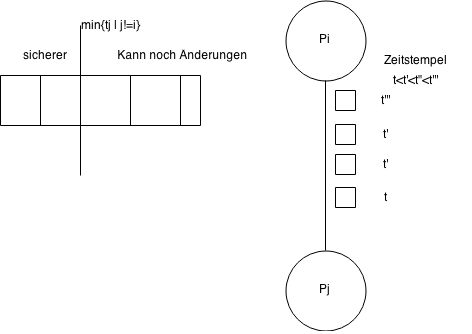
\includegraphics[scale=0.5]{lamport1.png}
\subsubsection{Matrix (Maekawa)}
Prozesse werden in einer Matrix angeordnet. Ein Knoten, der in einen kritischen Abschnitt eintreten will, sendet seinen Request an alle Knoten in seiner Zeile und seiner Spalte. Der Rest enspricht dem Lamport-Ansatz.\\
Deadlockrisiko, wenn ein Knoten dem einen ein OK gibt, während ein anderer den anderen Request akzeptiert. So ist zwar keiner der Requests im kritischen Abschnitt, aber beide warten wechselseitig auf den letzten Knoten. Kann durch Lamportzeit und Revoke-Antwort gelöst werden.\\
\subsubsection{Baum (Raymond)}
Die Wurzel des Baumes variiert, die Wurzel ist immer der Knoten, der das Token besitzt. Dadurch kennt jeder Knoten die Richtung zum Token (Wurzel).\\
Durch die vorgabe der Richtung zur Wurzel (über Eltern), ist es einfach einen Request für das Token an die Wurzel zu senden. Eltern, die nicht die Wurzel sind, geben den Request einfach an ihren Vater weiter.\\
Wenn ein Knoten, der bereits einen Request gesendet hat, einen weiteren Request weiterleiten soll, wird dieser nicht weitergeleitet, sondern gespeichert und in dem Moment beachtet, wenn der Knoten das Token hat. Wenn ein Knoten (auch das Token) über zwei Requests verfügt, wird jenes weitergeleitet, welches den kleineren Lamport-Zeitstempel besitzt. Das Token wird nun an diesen Knoten weitergeleitet, dazu kommt der Request, der nun noch nicht beantwortet wurde.

\subsubsection{Vergleich}
Die gegebenen Lösungen sind alle Optimal. Das geht, da sie alle eine andere Symmetriestufe bedienen. \\
Symmetrie beschreibt wie viele Knoten an der Bearbeitung eines Requests beteiligt sind. D.h., dass z.B. Maekawa Symmetrischer ist als Raymond, da immer eine gleiche Menge an Knoten per Request gefragt werden. Bei Raymond gibt es Knoten, die viel mehr Requests bearbeiten müssen, wenn sie höher in der Baumhierarchie sind.\\
Raymond wird für ein k welches gegen n konvergiert asymmetrischer, Maekawa wird symmetrischer.(K=Dimension (bei Baum Anzahl der direkten Kinder eines Knotens), n=Anzahl der Knoten).\\
Je größer die Symmetrie, desto redundanter ist das System, dafür steigt die Nachrichtenkomplexität. Bei einem sehr asymmetrischen System besteht die Gefahr eines SPOF/Bottleneck.\\
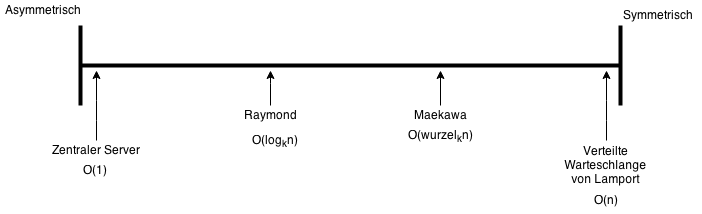
\includegraphics[scale=0.5]{Asymmetrisch.png}\\
%Lösungen mittels State-Variablen nicht relevant.
\section{Fehlertoleranz}
Fehlerklassen:
\begin{itemize}
\item[Crash] Systemausfall/Prozessausfall
\item[Ommission] 
\item[Timing] Antwort zu früh oder spät gesendet
\item[Arbitrary] Es ist nicht mehr sicher, ob die Antwort richtig ist, ungewollt
\item[Byzantinisch] Auch bewusste Falschantworten
\end{itemize}
Bis Timing wird davon ausgegangen, dass wenn eine Antwort kommt, ist sie richtig.
\subsection{Byzantinisch}
Zwei Armeen die hinter Hügeln auf zwei Seiten von Byzanz lagern, wollen dieses einnehmen, können es aber nur gemeinsam erreichen. Sie müssen sich also absprechen. Zum absprechen werden Boten geschickt. \\
A schickt B eine Nachricht mit einen weit genug in der Zukunft liegenden Termin. B schickt einen Boten zurück, der die Nachricht bestätigt. Nun weiß B nicht, ob die Nachricht angekommen ist. Es kann unendlich weiter Boten geschickt und Nachrichten bestätigt werden.\\
Fehlerfall: Ein Bote fällt aus.\\
Wenn man mit k Ausfällen rechnet, muss man mind. k+1 schicken, also redundanz.\\
Weiteres Problem: Nachricht kann kompromittiert werden (abgefangen und verändert).\\
Wenn man k gefälschte Nachrichten kompensieren möchte, muss A 2k+1 Nachrichten abschicken.\\
\subsection{Komponenten}
Das Kompensieren von Fehlern zieht sich durch alle Ebenen, das heißt, dass Software, Betriebssystem und Hardware Fehlerquellen sind.\\
Crash, Omission, Timing sind mit k+1 redundanten Maschinen kompensiert. Arbitrary benötigt 2k+1 redundante Maschinen, um per Mehrheitsentscheid die richtige Lösung herauszufinden.
\subsection{Lösungsansätze}
Passive Redundanz: Server schreibt Daten auf andere Datenspeicher. Backupserver können kontrollieren, ob der Server noch "lebt" und übernimmt, falls dieser ausfällt. Es sind nicht alle Fehlerklassen kompensierbar (nur die ersten 3 Klassen).\\
Aktive Redundanz: Client schickt Anfrage an eine Menge von Servern, und wählt durch Mehrheitsentscheid die richtige Antwort aus.
\subsection{Passive Redundanz}
Einfache Lösung mit mehreren Servern und ein Datenspeicher. STONITH Problem: Wennd er Primary Server nicht total ausfällt, sondern noch ab und zu Dateninkonsistenzen verursacht, muss der Backupserver den Primary selbst komplett abschalten.
\subsection{Aktive Redundanz}
\subsubsection{State-Machine-Approach}
Eine State-Machine Antwort hängt nur vom Startzustand und von der Reihenfolge der bearbeiteten Anfragen ab. Die meisten Server sind keine State-Machines, sie besitzen eigenes Verhalten. Nur bei State-Machines kann man die Antworten bitweise Vergleichen und auf Gleichheit prüfen.\\
Ein Voter sammelt und vergleicht die Antworten. Dieser Voter muss im Client liegen, da der Voter sonst ein SPOF ist.
\subsection{Fehlertoleranz in Multicast Netzwerken}
\subsection{Zuverlässigkeitsgrad}
\begin{itemize}
\item Keine Garantie, wieviele und welche Empfänger eine Nachricht erhalten.
\item Garantie, dass mindestens k Empfänger die Nachricht erhalten, wer diese Empfänger sind, ist u.U. bei jeder Nachricht unterschiedlich.
\item Garantie, dass entweder alle oder gar keine Nachricht ankommt.
\end{itemize}
\subsection{Ordnungsgrad}
Garantien über die Empfangsreihenfolge
\begin{itemize}
\item Keine Ordnungsgarantie
\item FIFO: Sender prüft, ob x+1 empfangen hat, wenn x bis dahin noch nicht empfangen hat, Fehler. Bei mehr als einem Client kann es zu Überschneidungen/Inkonsistenzen führen.
\item Kausale Ordnung, die Nachrichten kommen kausal korrekt an
\item Totale Ordnung, z.B. Lamport Zeit, aber schwer zu implementieren, da man globales Agreement braucht, welches bestimmte Zeitstempel einmalig macht.
\end{itemize}
Ethernetchips besitzen einen Cache für Multicast Adressen, Cache hat genug Platz für alle Adressgruppen.
\subsection{Überflutungsalgorithmen}
Über jede Kante soll maximal eine Nachricht versendet werden. Es wird ein Spannbaum aufgestellt (Baum der (minimal) alle Knoten verbindet).\\
\subsubsection{Echo-Algorithmus}
Der Sender schickt an allen von ihm ausgehenden Kanten die Nachricht. Die empfangenden Knoten nehmen die Nachricht an, und leiten sie an alle Kanten, außer der Empfangskante weiter. Knoten erkennen, wenn sie sich gegenseitig die selbe Nachricht geschickt haben (clash), diese Kante wird nicht mehr beachtet, sie ist nicht Teil des Spannbaums. Diese Knoten sind Blätter.\\
Blattknoten senden eine spezielle Antwort zurück. Innere Knoten können diese Antworten kombinieren und weiterleiten. 
\subsubsection{Amoeba-Multicast}
Dem Kern werden einzelne Unicast Nachrichten geschickt. Nur der Kern darf Multicasts senden (SPOF). Einige Empfängerknoten haben Sequencer, die Multicast Nachrichten empfangen. Die empfangenen Nachrichten werden nach Eingangsdatum sortiert. Es entsteht eine totale Ordnung. Ausfallende Sequencer können durch election ersetzt werden. Zuverlässigkeitsgrad von k setzt k+1 sequencer voraus. Das Verfahren hat einen konstanten Overhead von einer Unicast Nachricht.
\section{RPC und Client/Server}
\subsection{Realisierungen von Client/Server}
Zwei Möglichkeiten: Kommunikation ausgelagert in eigenen Kommunikationsserver oder kommunizierende Kerne.
\subsection{RPC}
Idee: Benutzer "bemerkt" Kommunikation nicht. 
Client sendet eine Nachricht an Empfänger, der daraufhin eine Methode ausführt und das Ergebnis zurück sendet. Client und Server Methodenstubs werden durch ein gegebenes Interface automatisch generiert.
\subsubsection{ONCPRC}
Generiert automatisch Code für Server und Client. Für die Funktion müssen nur die gewünschten Server-Methoden und die Client-Verbindungsdaten verändert werden. Zwischenstelle Portmapper, der von jedem Server dessen Port speichert. Der Client fragt diesen an.
\subsubsection{Probleme}
Ideal sollte RPC=LPC sein.\\
LPC wird nur unvollständig erreicht: Client muss Host angeben, Server sollten generell passiv sein, z.B. bei Pipes wird ein Server aber aktiv.\\
At-Most-Ansatz: Eine Aufgabe wird maximal 1 mal ausgeführt\\
At-Least-Ansatz: Eine Aufgabe wird minimal 1 mal ausgeführt\\
\underline{Zustandslose Server}
Client speichert den Zustand und sendet ihn dem Server mit (Sicherheitsproblem)\\
\underline{Idempotente Aufträge}
Eine Aufgabe die bei jeder Ausführung die selbe Antwort liefert.\\
\underline{Nicht-Idempotente Aufträge}
Kann in idempotente Aufträge verwandelt werden, indem alle Zustandsinformationen mitgeschickt werden.
\section{Verteilte Dateisysteme}
Dateisysteme sind für das persistente Speichern von Daten zuständig.\\
Merkmale: Blockzugriff, kleine Dateien, sequentieller Zugriff, nur wenige Daten von vielen verändert, meist nur von einem genutzt.\\
Update in Place (Spurwechsel bei Platte), Log (sequentiele Logfiles)\\
Grundlagen verteiltes FS: Durchsatz für Nutzer steigern, Skalierbarkeit, Zuverlässigkeit, Datenzugriff unabhängig von Aufenthaltsort.\\
\subsection{Transparenz}
\begin{itemize}
\item Zugangstransparenz: Identische Programmierschnittstelle
\item Ortstransparenz: Dateiort ist nicht ermittelbar
\item Namentransparenz: Dateiname ist überall gleich
\item Migrationstransparenz: Der Name bleibt auch bei Dateimigration gleich
\item Leistungstransparenz: Geschwindigkeit bei lokalen und entferntem Zugriff ist gleich
\item Fehlertransparenz: Fehler aufgrund der verteilten Architektur werden maskiert.
\end{itemize}
\subsection{Caching}
Daten werden gecached (Leistungssteigerung)\\
Bis zu ganze Dateien gecached, Read-ahead oder Seiten\\
\subsection{NFS}
Zugangstransparenz gegeben, Ortstransparenz je nach Konfiguration\\
Zustandslose Server, ausschließlich idempotente Operationen.\\
Caching auf Client- und Serverseite\\
Auf System wird ein Virtuelles Dateisystem über das UNIX Dateisystem gelegt, der NFS Client/Server ist teil dieses virtuellen FS. Das wird gemacht, damit man NFS Systeme auch verschachteln kann. Man kann also über NFS eine Datei öffnen, die auf dem Server auch nur per NFS eingebunden ist etc..\\
NFS verfügt über Dateideskriptor, obwohl zustandslos. Der Deskriptor muss unabhängig vom Serverzustand sein. Dieser Deskriptor ist kein Pfad, sondern eine ID von Server vergeben, um zu sehen, ob eine Datei verändert wurde.
\subsection{AFS - Andrew File System}
Skalierbarkeit mit mehr als 5000 Rechnern, Effizienz und Schutz.\\
Aufgeteilt in VICE (Server, als vertrauenswürdig betrachtet) und VENUS (Clients, UNIX)\\
Verfügt über Protection Domains (Benutzer- und Gruppenrechte), authentifizierung mit Kerberos\\
\subsection{Coda}
Ziel: Integration portabler Computer, gewollte Netzwerkpartitionierung, Kompensation von Server-/Netzwerkausfällen\\
Besitzt Konfliktlösungen.\\
Optimistische Replikation: Client arbeiten auf Dateien im eigenen Cache, Server behebt evtl. Konflikte\\
Replikation bestimmter Teile des gemeinsamen Systems in einer Volume Storage Group\\
Periodische Tests prüfen Accessible VSG (AVSG), Preferred Server wird ausgewählt, bei Ausfall wird ein neuer aufgenommen\\
\subsubsection{Disconnected Operation}
AVSG = $\emptyset$\\
Optimistisch: Venus arbeitet auf Cache\\
Hoarding: Soviel wir möglich lokal cachen, Venus beobachtet Zugriffe\\
Emulation: Venus übernimmt Serverrolle, Reply-Log aufzeichnen, Kritische Daten in Recoverabel Virtual Memory speichern\\
Reintegration: Reply-Log an AVSG übergeben, der dann verarbeitet; Viele Konflikte automatisch lösbar, rest manuell\\
Hoarding $\rightarrow$ Emulation $\rightarrow$ Reintegration $\rightarrow$ Hoarding\\
\subsubsection{Surrogate}
Mobile Geräte sind unzuverlässig (Netzwerk), gerine Rechenleistung\\
Operation Shipping: Statt Datenblöcke werden Replay-Operationen and Surrogate gesendet, Surrogate aktualisiert Server\\
\subsection{ZEBRA}
Network RAID, riesige Logfile, Schreiben IMMER an Anfang, Stripe Cleaner schreibt sehr alte Blöcke vorne an. Damit wird hinten das "Band" frei.\\
Klappt IMMER! (Technische Details)\\
\subsection{P2P-Dateisysteme}
Verteiltes Speichern von Dateien, damti überall verfügbar, Leistung und Fehlertoleranz\\
Probleme: Peers können jederzeit offline gehen, keine unverschlüsselte Speicherung\\
\subsubsection{Self-*}
Self-organizing: Keine Zentrale administration\\
Self-repairing: Reparatur von Lücken automatisch (z.B. Weggang von Ressourcen)\\
Self-tuning: Optimierung über Zeit z.B. verbesserung der Latenz\\
\subsection{Tapestry}
Routing über Namen unabh. vom Aufenthaltsort\\
DHT: Distributed Hash Table (Name wird gehashed, möglichst keine duplikate)\\
Stationen bekommen eine ID (z.B. auch durch Hashes), werden nach ID aufsteigend als Ring aufgebaut\\
Stationen sollen Daten speichern, Daten haben Namen und auch Hash. Eine Datei wird auf der Station gespeichert, deren ID näher an der der Datei  ist. Stationen können das unter sich aushandeln, da sie die ID und die Richtung kennen. Eine neue Station handelt mit Nachbarn die zu übernehmenden Daten aus.\\
Von jedem Knoten aus gibt es ein paar Kanten, die große Teile des Rings überspringen. Falls sich die DatenID stark von der eigenen unterscheidet, wird es an eine völlig andere Stelle des Rings weitergegeben.\\
Damit Stationen ausfallen können gibt es Replikate, deren Name sich aus dem Namen der Originaldatei ableiten lässt, diese liegt dann auf einem anderen Server.
\end{document}

